\documentclass[conference]{IEEEtran}
\IEEEoverridecommandlockouts
% The preceding line is only needed to identify funding in the first footnote. If that is unneeded, please comment it out.
\usepackage{cite}
\usepackage{amsmath,amssymb,amsfonts}
\usepackage{algorithmic}
\usepackage{graphicx}
\usepackage{textcomp}
\usepackage{xcolor}
\def\BibTeX{{\rm B\kern-.05em{\sc i\kern-.025em b}\kern-.08em
    T\kern-.1667em\lower.7ex\hbox{E}\kern-.125emX}}
\begin{document}

\title{Real-Time Monitoring and Remote Guidance of\\ Mobile Robots Using Multimodal Digital Twins}

\author{\IEEEauthorblockN{Trung Kien La}
\IEEEauthorblockA{\textit{Dept. of Comp. Science \& Engineering} \\
\textit{Frankfurt University of Applied Sciences}\\
Frankfurt a.M., Germany \\
trung.la@stud.fra-uas.de}
\and
\IEEEauthorblockN{René Harmann}
\IEEEauthorblockA{\textit{Dept. of Comp. Science \& Engineering} \\
\textit{Frankfurt University of Applied Sciences}\\
Frankfurt a.M., Germany\\
rene.harmann@fb2.fra-uas.de}
\and
\IEEEauthorblockN{Eric Guiffo Kaigom}
\IEEEauthorblockA{\textit{Dept. of Comp. Science \& Engineering} \\
\textit{Frankfurt University of Applied Sciences}\\
Frankfurt a.M., Germany \\
kaigom@fb2.fra-uas.de}

}

\maketitle

\begin{abstract}
    Although digital twins have been playing a pivotal
    role in the management of the lifecycle of physical robotic
    systems of systems, they have hardly been employed to guide
    mobile robots in real-time. In fact, the guidance of such systems
    requires functionalities, including the perception of targeted
    locations and avoidance of collisions, that build upon spatial
    information beyond internal robot states usually acquired using
    proprioceptive sensors. In this case, exteroceptive sensors help
    meet this demand. Nevertheless, such sensors have received little
    attention thus far in the development of digital twins. On the
    other hand, the completion of various spatial objectives, such as
    reverse motions, might require the awareness of the historical
    internal state of the distant robot. For instance, the current
    energy budget is likely to constrain the reachability of the
    initial state after a while, even when spatially and kinematically
    feasible. We therefore embrace these challenges with a multi-
    modal approach to provide and employ digital twin of mobile
    robots. We collect data about the internal state and camera-
    captured neighborhood of the robot in real-time. The robot
    operator is thereby provided with a multi-dimensional state and
    perception view that characterizes the robot, elevates situational
    awareness, and facilitates decision support. We then develop a
    versatile graphical interface that helps monitor and steer mobile
    robots. Since the bidirectional approach is intuitive and user
    friendly, even novices can remotely guide a mobile robot with
    multi-modal situational awareness. We show the versatility and
    effectiveness of our approach in use case scenarios in practice.
\end{abstract}

\begin{IEEEkeywords}
    Robotics, Multimodal Data, Digital Twins, In-
    dustry 4.0, Industry 5.0, Society 5.0, Human-Mobile Robot-
    Interaction, Systems of Systems
\end{IEEEkeywords}

\section{Introduction}
The Robot Operating System (ROS) stands as a ubiquitous middleware framework in the realm of robotics, serving as a foundational platform for constructing robot systems and developing robot applications. 
However, for individuals possessing limited or no prior exposure to robot software, navigating the intricacies of ROS can prove challenging. 
This challenge is particularly pronounced for users who rely on robotic assistance and require an intuitive means of interacting with these machines.
In response to this need, a platform-independent web application was meticulously crafted. 
Designed with accessibility in mind, this application facilitates seamless monitoring and control of locally networked robots. Users gain access to critical information, including battery status and motor temperatures, all presented through an intuitive web interface. 
Notably, this application is compatible with any device supporting web browsers, ensuring widespread accessibility and usability.
\begin{figure}[htbp]
    \centerline{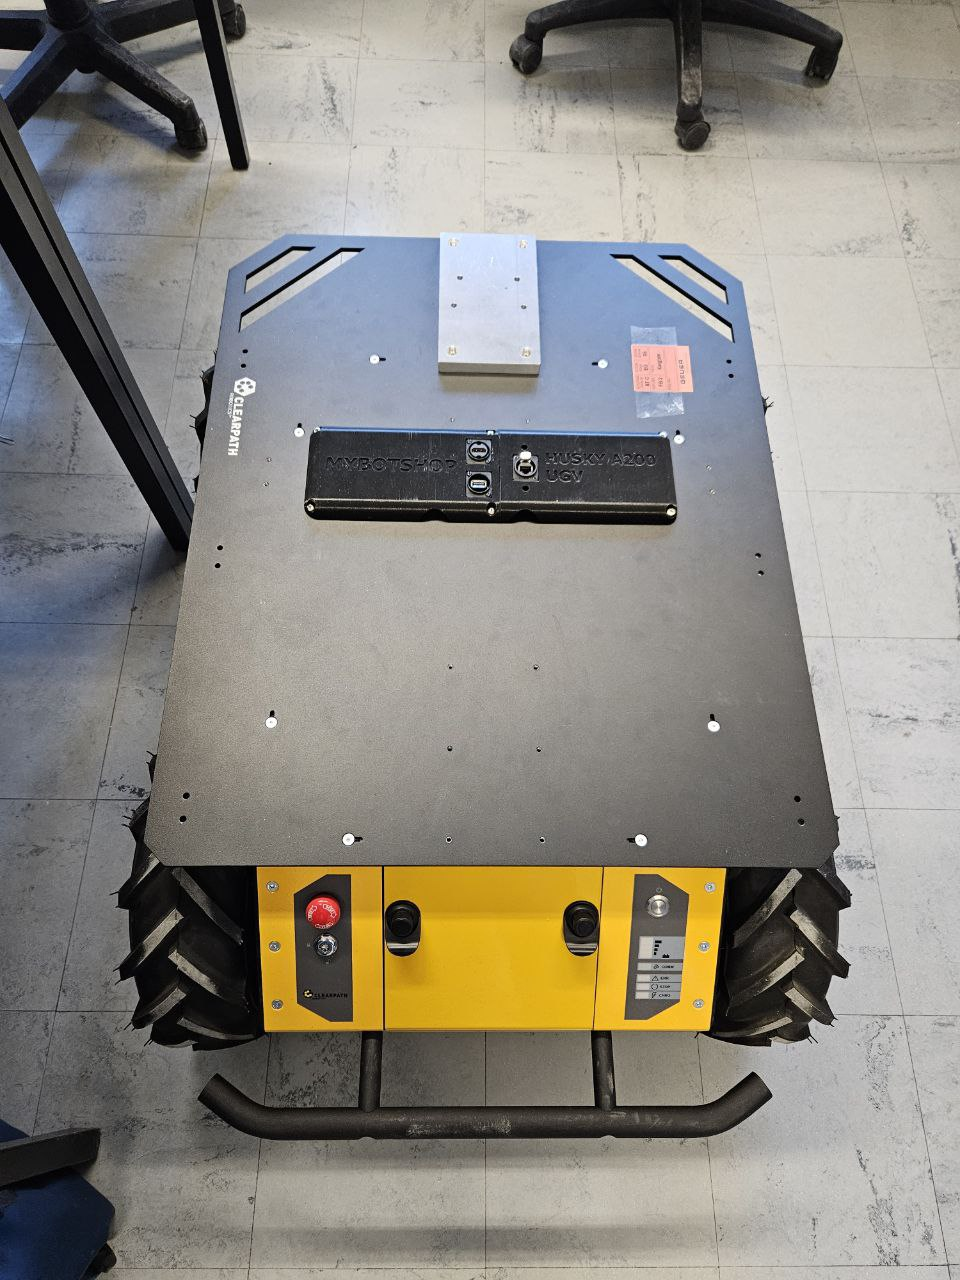
\includegraphics[width=8.9cm]{Pictures/husky_costum.jpeg}}
    \caption{Picture of the Husky UGV by Clearpath}
    \label{fig:huskyClearpath}
\end{figure} 
The robotic platform employed in our research is the Husky Unmanned Ground Vehicle (UGV), manufactured by Clearpath Robotics. This medium-sized mobile robot, depicted in Fig. \ref{fig:huskyClearpath}, operates on the ROS2 distribution Humble Hawksbill.
The Husky UGV boasts a substantial maximum payload capacity of 75 kg, rendering it suitable for transporting and accommodating various auxiliary components. Researchers can mount additional robots, peripherals, and specialized tools on this versatile platform. Its robust design and adaptability make it an ideal choice for a wide range of robotic applications\cite{huskyClearpath}. 




\section{State of the Art}
C. Crick et al.  
\begin{itemize}
\item r
\item teams
\item s
\end{itemize}

\subsection{placeholder}
placeholder

\section{Implementation and Design}
The system architecture of the web application can be dichotomized into distinct backend and frontend components. These components synergistically leverage an array of tools and frameworks to facilitate seamless operation.
\subsection{Backend}
The web application is a Flask application. Flask is a micro web framework that is characterized by providing the core features to create a python web based application. 
Flask is also very flexible and highly expandable \cite{flasksqlite}. The following tools are used in the backend:
\begin{itemize}
\item SQLAlchemy is a Python SQL toolkit and can be integrated into Flask as an extension. SQLAlchemy allows users to link Python objects to SQL databases using Object-Relational Mapping (ORM). This allows, for example, database queries to be made using Python code instead of SQL commands. The extension is also database-agnostic. 
Python code can be used unchanged for various SQL-based databases, such as SQLite, PostgreSQL or MySQL. 
SQLite3 is used as a database to store ROS and user data. SQLite3 is a serverless database. This characteristic renders it operable in a self-contained manner, devoid of any supplementary software dependencies or intricate configuration settings. Consequently, it exhibits resource efficiency by minimizing the utilization of extraneous computational resources.
\item The Roslibjs JavaScript library and the Rosbridge v2.0 protocol are used to establish bidirectional communication with the robots and the web application. The Rosbridge server it contains, provides a WebSocket connection so that web browsers can communicate with Rosbridge.
Roslibjs is employed as a JavaScript library to interact with ROS topics, enabling the subscription to and publication of these topics. A quintessential example of this interaction is the publication of a geometry\_msgs/Twist message on the /cmd\_vel topic of the Husky robot, which initiates its movement.
The geometry\_msgs/Twist message is composed of linear and angular vectors, which represent the velocity in free space. Specifically, these vectors are expressed in terms of m/s and rad/s, respectively, in a right-handed coordinate system.
In the context of the Husky robot, a linear velocity of 1 m/s in the positive x-direction corresponds to forward movement at a speed of 1 m/s. To induce rotational movement, an angular velocity is specified in the z-direction. Positive and negative values correspond to counterclockwise and clockwise rotations, respectively.
\item The Web Video Server is a ROS package that allows HTTP streaming of ROS image topics. This integrates the live image from a Zed 2i camera from StereoLabs into the web interface.
\item Flask-Login and Werkzeug.security extensions are used to handle login, logout, and session functions, as well as to enhance user password security through password hashing.
\end{itemize}
\begin{figure}[htbp]
    \centerline{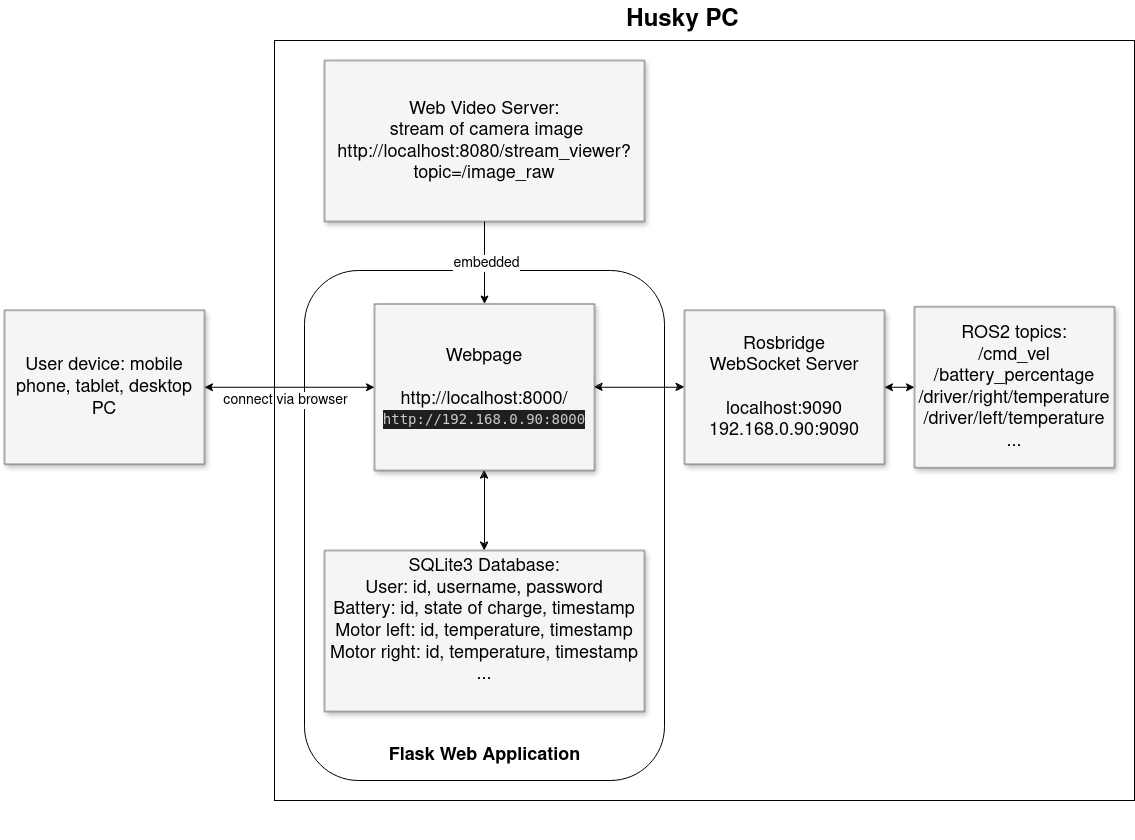
\includegraphics[width=8.9cm]{Pictures/userapp.png}}
    \caption{Backend architecture of the web app}
    \label{fig:userapp}
\end{figure}
Fig. \ref{fig:userapp} illustrates the backend architecture and the method by which users can interface with the Husky robot via the web application. This system is designed to operate on any device equipped with a web browser, utilizing the IP address of the Husky's onboard computer for connectivity.
The user interface provides real-time access to a stream of visual data from a Zed 2i camera, as well as control options for the robot. Additionally, it displays current ROS data, including metrics such as the battery state of charge (soc) and motor temperatures.
A key feature of this system is its ability to track and store historical data in the SQLite3 database. This allows for longitudinal analysis of the robot's operational data, which can be instrumental in performance optimization and troubleshooting.
This system provides a flexible and accessible platform for robot control and data monitoring. It underscores the potential of web-based interfaces in enhancing the usability and functionality of robotic systems. 
The use of an IP-based connection protocol further emphasizes the system's adaptability and broad accessibility. The incorporation of a database for data tracking and storage demonstrates a commitment to data-driven decision making and performance optimization. 
\subsection{Frontend}
The primary objective of the front-end design is to enhance user-friendliness through visually intuitive elements. Additionally, the application aims for robust platform independence, ensuring that users are not constrained by specific devices when accessing the web user interface. 
To achieve this, the web application is meticulously crafted to be compatible with a wide range of devices, including desktop PCs and mobile platforms. 
\begin{itemize}
\item Leveraging the free and open-source CSS framework Bootstrap version 4.6, we optimize responsiveness and seamlessly integrate with prevailing web standards such as HTML5, CSS3, and JavaScript. 
In the context of Bootstrap, the layout structure is organized using the grid system, for arranging elements within a web page. 
Additionally, a navigation bar is crafted to reinforce user navigation.
Furthermore, the implementation of a battery display is achieved through the utilization of the Bootstrap class .progress-bar. 
This class enables precise control over visual representations of battery levels or other progress indicators.
\item Plotly.js, an open-source graphing library, serves as a powerful tool for constructing interactive and touch-enabled visualizations. It facilitates the creation of dynamic plots that allow users to zoom in and out, as well as capture screenshots of relevant data.
\item The Husky is supplied with a physical controller as standard. Teleoperation is achieved through the utilization of an analog joystick and the left and right shoulder buttons to set a specific maximum velocity.
To extend this functionality to the web interface, Nipple.js is employed. This library empowers the configuration and display of a virtual joystick. Additionally, a horizontally scrollable velocity slider is created using the Bootstrap class .form-control-range to set the maximum speed.
\item The app exhibits versatility in its control mechanisms. Users have the option to teleoperate the robot via a physical keyboard, provided they have one readily available. For users lacking a physical keyboard connection, an alternative method involves utilizing the “WASD” touch keys displayed within the application interface. 
These touch keys can also be used for the robot movement. The Huksy can be driven more precisely using the keyboard buttons. This can be useful when parking, for instance.
\end{itemize}


\subsection{Examples backend and frontend}

\subsection{\LaTeX-Specific Advice}



\subsection{Some Common Mistakes}

\begin{thebibliography}{00}
\bibitem{rosOrg} “ros.org,”
2024.
[Online].
Available:
https://ros.org
\bibitem{huskyClearpath} “clearpathrobotics.com,”
2024.
[Online].
Available:
https://clearpathrobotics.com/husky-unmanned-ground-vehicle-robot/
\bibitem{rosbridgeOkState} Crick, C., Jay, G., Osentoski, S., Pitzer, B., and Jenkins, O. C. ``Rosbridge: Ros
for non-ros users,'' in Robotics Research, Springer, 2017, pp. 493--504.
\bibitem{flasksqlite} Suraya, Muhammad Sholeh, ``Designing and Implementing a Database for Thesis Data,'' in International Journal of Engineering, Science \& InformationTechnology (IJESTY)
Volume 2, No. 1, 2022, pp. 9--14, eISSN: 2775-2674
\bibitem{rosbridgeSuite}“ros.org,” 
2024.
[Online]. 
Available:
http://wiki.ros.org/rosbridge\_suite
\end{thebibliography}
\vspace{12pt}
\color{red}
IEEE conference templates contain guidance text for composing and formatting conference papers. Please ensure that all template text is removed from your conference paper prior to submission to the conference. Failure to remove the template text from your paper may result in your paper not being published.

\end{document}
